%\mypartheader{Publications}
\section{Publications}
\noindent My work has been published in several prestigious journals and international conferences, including: 
\begin{itemize}
	\itemsep-0.2em
	
	\item Information Systems  (IS) -- 6x
	
	\item Decision support systems (DSS) -- 2x
	
	\item IEEE Transactions on Knowledge and Data Engineering (TKDE) -- 1x
	
	\item Data and Knowledge Engineering  (DKE) -- 2x
	
	\item Int.\ Conf.\ on Advanced Information Systems Engineering (CAISE)	 -- 7x
	
	\item Int.\ Conf.\ on Business Process Management (BPM) --  5x

	\item Int.\ Conf.\ on Computational Linguistics (COLING) -- 1x
	
	\item ACM Int.\ Conf.\ on Management of Data (SIGMOD) -- 1x 
	
	
\end{itemize}
\smallskip
Pre-print versions of all my publications are available at \href{https://www.hanvanderaa.com/publications}{www.hanvanderaa.com/publications}\\

%\section{Bibliographic Profile}
%\begin{figure}[!h]
%	\centering
%	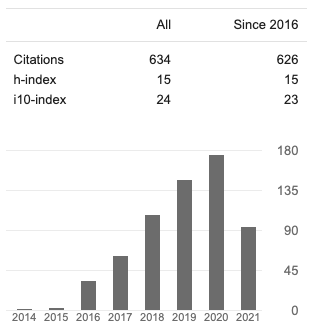
\includegraphics[width=0.38\linewidth]{figures/scholarprofile.png}
%\end{figure}
%
%Updated:  June 29, 2021 (source: \href{https://scholar.google.com/citations?user=oFagE6cAAAAJ}{scholar.google.com/citations?user=oFagE6cAAAAJ})\\

\section{Selected Publications}

\begin{enumerate}[label=\arabic*.]
	\itemsep-0.3em
	\mybib{\textbf{Han van der Aa}, Adrian Rebmann, Henrik Leopold}
	{Natural language-based detection of semantic execution anomalies in event logs}
	{Information System 102: 101824, 2021}
	
			\mybib{ Bo Zhao, \textbf{Han van der Aa}, Nguyen Thanh Tam, Nguyen Quoc Viet Hung, Matthias Weidlich} {EIRES Efficient Integration of Remote Data in Event Stream Processing}
	{ACM SIGMOD International Conference on Management of Data (SIGMOD 2021)}
	
	\mybib{ Adrian Rebmann, \textbf{Han van der Aa}} {Extracting Semantic Process Information from the Natural Language in Event Logs} 
	{International Conference on Advanced Information Systems Engineering (CAiSE 2021)}
	
	\mybib{Martin Bauer, \textbf{Han van der Aa}, Matthias Weidlich}
	{Sampling and Approximation Techniques for Efficient Process Conformance Checking}
	{Information Systems 2020 (accepted for publication)}
	
	\mybib{\textbf{Han van der Aa}, Henrik Leopold, Matthias Weidlich}
	{Partial Order Resolution of Event Logs for Process Conformance Checking}
	{Decision Support Systems 136: 113347, 2020}



	\mybib{\textbf{Han van der Aa}, Henrik Leopold, Hajo A. Reijers}{Efficient Process Conformance Checking on the Basis of Uncertain Event-to-Activity Mappings}
{IEEE Transactions on Knowledge and Data Engineering  32(5): 927-940, 2020}

	\mybib{ Stephan A Fahrenkrog-Petersen, \textbf{Han van der Aa}, Matthias Weidlich} {	PRIPEL: Privacy-Preserving Event Log Publishing Including Contextual Information}
{International Conference on Business Process Management (BPM 2020)}

	\mybib{ \textbf{Han van der Aa}, Claudio Di Ciccio, Henrik Leopold and Hajo A Reijers} {Extracting Declarative Process Models from Natural Language} 
{International Conference on Advanced Information Systems Engineering (CAiSE 2019)}
	
\mybib{\textbf{Han van der Aa}, Henrik Leopold, Hajo A. Reijers}{Comparing Textual Descriptions to Process Models – The Automatic Detection of Inconsistencies}
{Information Systems 64: 447-460, 2017}

\mybib{ Claudio Di Ciccio, \textbf{Han van der Aa}, Cristina Cabanillas, Jan Mendling, Johannes Prescher}{Detecting Flight Trajectory Anomalies and Predicting Diversions in Freight Transportation}
{Decision Support Systems 88(1): 1-17, 2016}

\end{enumerate}
%\section{Journal Articles}


%\begin{enumerate}[label=J\arabic*.]
%	\itemsep-0.3em
%	\mybib{\textbf{Han van der Aa}, Adrian Rebmann, Henrik Leopold}
%	{Natural language-based detection of semantic execution anomalies in event logs}
%	{Information System 102: 101824, 2021}
%	
%	
%	\mybib{Martin Bauer, \textbf{Han van der Aa}, Matthias Weidlich}
%	{Sampling and Approximation Techniques for Efficient Process Conformance Checking}
%	{Information Systems 2020 (accepted for publication)}
%	
%	\mybib{\textbf{Han van der Aa}, Henrik Leopold, Matthias Weidlich}
%	{Partial Order Resolution of Event Logs for Process Conformance Checking}
%	{Decision Support Systems 136: 113347, 2020}
%
%		\mybib{Nimrod Busany, \textbf{Han van der Aa}, Arik Senderovich, Avigdor Gal, Matthias Weidlich}
%{Interval-based Queries over Lossy IoT Event Streams}
%{ACM Transactions on Data Science 1(4): 27:1-27:27, 2020}
%	
%	\mybib{\textbf{Han van der Aa}, Henrik Leopold, Hajo A. Reijers}{Efficient Process Conformance Checking on the Basis of Uncertain Event-to-Activity Mappings}
%	{IEEE Transactions on Knowledge and Data Engineering  32(5): 927-940, 2020}
%	
%	
%	
%	\mybib{ Henrik Leopold, \textbf{Han van der Aa}, Jelmer Offenberg, Hajo A. Reijers}{Using Hidden Markov Models for the Accurate Linguistic Analysis of Process Model Activity Labels} {Information Systems 83: 30-39, 2019}
%	
%	\mybib{ Henrik Leopold, \textbf{Han van der Aa}, Fabian Pittke, Manuel Raffel, Jan Mendling, Hajo A. Reijers}{Searching Textual and Model-based Process Descriptions based on a Unified Data Format}
%	{Software and Systems Modeling, 18(2):1179-1194, 2019}
%	
%	\mybib{ Josep S\'anchez-Ferreres, \textbf{Han van der Aa}, Josep Carmona, Llu\'is Padro}{Aligning Textual and Model-Based Process Descriptions}
%	{Data \& Knowledge Engineering, 118:24-40, 2018}
%	
%	\mybib{ Elena Kuss, Henrik Leopold, \textbf{Han van der Aa}, Heiner Stuckenschmidt, Hajo A. Reijers} {A Probabilistic Evaluation Procedure for Process Model Matching Techniques}
%	{Data \& Knowledge Engineering, 117:393-406, 2018}
%	
%	\mybib{ \textbf{Han van der Aa}, Henrik Leopold, Hajo A. Reijers}{Checking Process Compliance against Natural Language Specifications using Behavioral Spaces}
%	{Information Systems, 78:83-95, 2018}
%	
%	
%	\mybib{ \textbf{Han van der Aa}, Henrik Leopold, Adela del-Rio-Ortega, Manuel Resinas, Hajo A. Reijers}
%	{Transforming Unstructured Natural Language Descriptions into Measurable Process Performance Indicators Using Hidden Markov Models}
%	{Information Systems 71:27-39, 2017}
%	
%	\mybib{\textbf{Han van der Aa}, Henrik Leopold, Hajo A. Reijers}{Comparing Textual Descriptions to Process Models – The Automatic Detection of Inconsistencies}
%	{Information Systems 64: 447-460, 2017}
%	
%	\mybib{ Claudio Di Ciccio, \textbf{Han van der Aa}, Cristina Cabanillas, Jan Mendling, Johannes Prescher}{Detecting Flight Trajectory Anomalies and Predicting Diversions in Freight Transportation}
%	{Decision Support Systems 88(1): 1-17, 2016}
%	
%	\mybib{ \textbf{Han van der Aa}, Hajo A. Reijers, Irene Vanderfeesten}{Designing Like a Pro: The Automated Composition of Workflow Activities}
%	{Computers in Industry 75(1): 162-177, 2016}
%	
%	
%\end{enumerate}
%
%\section{Conference Proceedings}
%
%\begin{enumerate}[label=C\arabic*.]
%	\itemsep-0.3em
%	
%		\mybib{ Bo Zhao, \textbf{Han van der Aa}, Nguyen Thanh Tam, Nguyen Quoc Viet Hung, Matthias Weidlich} {EIRES Efficient Integration of Remote Data in Event Stream Processing}
%	{ACM SIGMOD International Conference on Management of Data (SIGMOD 2021)}
%	
%	\mybib{ Adrian Rebmann, \textbf{Han van der Aa}} {Extracting Semantic Process Information from the Natural Language in Event Logs} 
%	{33rd International Conference on Advanced Information Systems Engineering (CAiSE 2021)}
%		
%	\mybib{ Bernhard Sch\"afer, \textbf{Han van der Aa}, Henrik Leopold, Heiner Stuckenschmidt} {Sketch2BPMN: Automatic Recognition of Hand-drawn BPMN Models}
%	{33rd International Conference on Advanced Information Systems Engineering (CAiSE 2021)}
%
%	\mybib{ Diana Sola, Christian Meilicke, \textbf{Han van der Aa}, Heiner Stuckenschmidt} {A Rule-based Recommendation Approach for Business Process Modeling}
%	{33rd International Conference on Advanced Information Systems Engineering (CAiSE 2021)}
%	
%	\mybib{ 	Karolin Winter, \textbf{Han van der Aa}, Stefanie Rinderle-Ma, Matthias Weidlich} {	Assessing the Compliance of Business Process Models with Regulatory Documents}
%	{39th International Conference on Conceptual Modeling (ER 2020)}
%	
%	\mybib{ Stephan A Fahrenkrog-Petersen, \textbf{Han van der Aa}, Matthias Weidlich} {	PRIPEL: Privacy-Preserving Event Log Publishing Including Contextual Information}
%	{18th International Conference on Business Process Management (BPM 2020)}
%	
%	\mybib{ 	Martin Bauer, \textbf{Han van der Aa}, Matthias Weidlich} {	Estimating Process Conformance by Trace Sampling and Result Approximation}
%	{17th International Conference on Business Process Management (BPM 2019)}
%	
%	\mybib{ Stephan A Fahrenkrog-Petersen, \textbf{Han van der Aa} and Matthias Weidlich} {PRETSA: Event Log Sanitization for Privacy-aware Process Discovery} 
%	{1st International Conference on Process Mining (ICPM 2019)}
%	
%	\mybib{ \textbf{Han van der Aa}, Claudio Di Ciccio, Henrik Leopold and Hajo A Reijers} {Extracting Declarative Process Models from Natural Language} 
%	{31st International Conference on Advanced Information Systems Engineering (CAiSE 2019)}
%	
%	\mybib{  \textbf{Han van der Aa}, Josep Carmona, Henrik Leopold, Jan Mendling, Lluis Padro} {Challenges and Opportunities of Applying Natural Language Processing in Business Process Management} 
%	{27th International Conference on Computational Linguistics (COLING 2018)}
%	
%	\mybib{ \textbf{Han van der Aa}, Henrik Leopold, Inge van de Weerd, Hajo A Reijers} {Causes and Consequences of Fragmented Process Information: Insights from a Case Study} 
%	{23rd Americas Conference on Information Systems (AMCIS 2017)}
%	
%	\mybib{ \textbf{Han van der Aa}, Avigdor Gal, Henrik Leopold, Hajo A Reijers, Tomer Sagi, Roee Shraga} {Instance-Based Process Matching using Event-Log Information} 
%	{29th International Conference on Advanced Information Systems Engineering (CAiSE 2017)}
%	
%	\mybib{ \textbf{Han van der Aa}, Henrik Leopold, Hajo A Reijers} {Checking Process Compliance on the Basis of Uncertain Event-to-Activity Mappings} 
%	{29th International Conference on Advanced Information Systems Engineering (CAiSE 2017)}
%	
%	\mybib{ Elena Kuss, Henrik Leopold, \textbf{Han van der Aa}, Heiner Stuckenschmidt, Hajo A Reijers} {Probabilistic Evaluation of Process Model Matching Techniques} 
%	{35th International Conference on Conceptual Modeling (ER 2016)}
%	
%	\mybib{ \textbf{Han van der Aa}, Henrik Leopold, Hajo A Reijers} {Dealing with Behavioral Ambiguity in Textual Process Descriptions} 
%	{14th International Conference on Business Process Management (BPM 2016)}
%	
%	\mybib{ Ermeson Andrade, \textbf{Han van der Aa}, Henrik Leopold, Steven Alter, Hajo A Reijers} {Factors Leading to Business Process Noncompliance and its Positive and Negative Effects: Empirical Insights from a Case Study}
%	{22nd Americas Conference on Information Systems (AMCIS 2016)}
%	
%	\mybib{ \textbf{Han van der Aa}, Adela del-Rio-Ortega, Manuel Resinas, Henrik Leopold, Antonio Ruiz-Cortés, Jan Mendling, Hajo A Reijers} 
%	{Narrowing the Business-IT Gap in Process Performance Measurement} 
%	{28th International Conference on Advanced Information Systems Engineering (CAiSE 2016)}
%	
%	\mybib{ \textbf{Han van der Aa}, Henrik Leopold, Hajo A Reijers} {Detecting Inconsistencies between Process Models and Textual Descriptions} 
%	{13th International Conference on Business Process Management (BPM 2015)}
%	
%	\mybib{ \textbf{Han van der Aa}, Hajo A Reijers, Irene Vanderfeesten} {Composing Workflow Activities on the Basis of Data-flow Structures} 
%	{11th International Conference on Business Process Management (BPM 2013)}
%\end{enumerate}
%
%\section{Book}
%
%\begin{enumerate}[label=B\arabic*.]
%	
%	\mybib{\textbf{Han van der Aa}}
%	{Comparing and Aligning Process Representations: Foundations and Technical Solutions} {Lecture Notes on Business Information Processing (LNBIP), Vol. 323, Springer-Verlag, 2018}
%	
%\end{enumerate}
%
%\section{Book Chapters}
%
%\begin{enumerate}[label=Ch\arabic*.]
%	\itemsep-0.2em
%	\mybib{Henrik Leopold and \textbf{Han van der Aa} }
%	{Automatically Identifying Process Automation Candidates Using Natural Language Processing}
%	{Blockchains \& RPA, Springer (forthcoming, 2021)}
%	
%	
%	\mybib{\textbf{Han van der Aa} and Henrik Leopold}
%	{Supporting Robotic Process Automation through Natural Language Processing}
%	{Robotic Process Automation, De Gruyter STEM (2021)}
%	
%	\mybib{\textbf{Han van der Aa}, Alexander Artikis, Matthias Weidlich}
%	{Complex Event Processing Methods for Process Querying}
%	{Process Querying Methods (forthcoming, 2021)}
%	
%\end{enumerate}
%
%\section{Workshop and Working Conference Proceedings}
%\begin{enumerate}[label=W\arabic*.]
%	\itemsep-0.3em
%	
%	\mybib{ Anti Alman, Karl Johannes Balder, Fabrizio M. Maggi, \textbf{Han van der Aa}}
%{Declo: A Chatbot for User-friendly Specification of Declarative Process Models}
%	{18th International conference on Business Process Management (BPM Demos 2020)}
%	
%	\mybib{\textbf{Han van der Aa}, Karl Johannes Balder, Fabrizio M. Maggi, Alexander Nolte}
%{Say It In Your Own Words: Defining Declarative Process Models Using Speech Recognition}
%	{18th International conference on Business Process Management (BPM Forum 2020)}
%	
%	\mybib{	Martin Bauer, Stephan A. Fahrenkrog-Petersen, Agnes Koschmider, Felix Mannhardt, \textbf{Han van der Aa}, Matthias Weidlich} 
%	{ELPaaS: Event Log Privacy as a Service}
%	{17th International Conference on Business Process Management (BPM Demos 2019)}
%
%	\mybib{ Jan Mendling, Henrik Leopold, Lucinéia Heloisa Thom, \textbf{Han van der Aa}}
%	{Natural Language Processing with Process Models} 
%	{2nd Workshop on Natural Language Processing for Requirements Engineering \& NLP}
%%
%	\mybib{ Michael Offel, \textbf{Han van der Aa}, Matthias Weidlich}
%	{Towards Net-based Formal Methods for Complex Event Processing}
%	{Large-scale Data Management and Processing – Applications in Research and Industry (LWDA 2018)}
%	
%	\mybib{Henrik Leopold, \textbf{Han van der Aa}, Hajo A. Reijers}
%	{Identifying Candidate Tasks for Robotic Process Automation in Textual Process Descriptions} {BPMDS’18 Working Conference (BPMDS 2018)}
%	
%	\mybib{ Henrik Leopold, \textbf{Han van der Aa}, Fabian Pittke, Manuel Raffel, Jan Mendling, Hajo A. Reijers}
%	{Integrating Textual and Model-based Process Descriptions for Comprehensive Process Search} {BPMDS’16 Working Conference (BPMDS 2016)}
%	
%	\mybib{ \textbf{Han van der Aa}, Henrik Leopold, Kimon Batoulis, Mathias Weske, Hajo A. Reijers} {Integrated Process and Decision Modeling for Data-Driven Processes}
%	{3th International Workshop on Decision Mining \& Modeling for Business Processes (DeMiMoP’15)}
%	
%	\mybib{ \textbf{Han van der Aa}, Henrik Leopold, Felix Mannhardt, Hajo A. Reijers}
%	{On the Fragmentation of Process Information: Challenges, Solutions, and Outlook}
%	{BPMDS’15 Working Conference (BPMDS 2015)}
%	
%\end{enumerate}

